\section{Auswertung}
\label{sec:Auswertung}

Im folgenden wird auf drei verschiedene Arten die Zeitkonstante $RC$ bestimmt. 
Außerdem wird die Integration von drei Spannungen dargestellt.

\subsection{Bestimmung der Zeitkonstanten durch Beobachtung des Entladevorgangs des Kondensators}
Es werden bei einer angelegten Rechteckspannung die Spannung $U_c$ und die zugehörige Zeit $t$ gemessen.
Für eine lineare Ausgleichsrechnung wird der Logarithmus der Spannung berechnet, und dieser wird gegen t aufgetragen.
Alle Werte sind in Tabelle (1) aufgelistet. Der Wert für $U_0$ beträgt 18 V.

\noindent Der Ansatz der linearen Regression lautet
\begin{equation}
    y = ax+b .
\end{equation}
%Die Werte für $a$ und $b$ bestimmen sich folgendermaßen:
%\begin{align}
%a = \frac{\overline{xy}-\overline{x}\cdot\overline{y}}{\overline{x^2}-\overline{x}^2}, \\
%  b = \frac{\overline{x^2}\overline{y}-\overline{xy}\cdot\overline{x}}{\overline{x^2}-\overline{x}^2} .
%\end{align}
Der Plot, die Parameter und die Fehler werden mit Python berechnet.

\begin{figure}
  \centering
  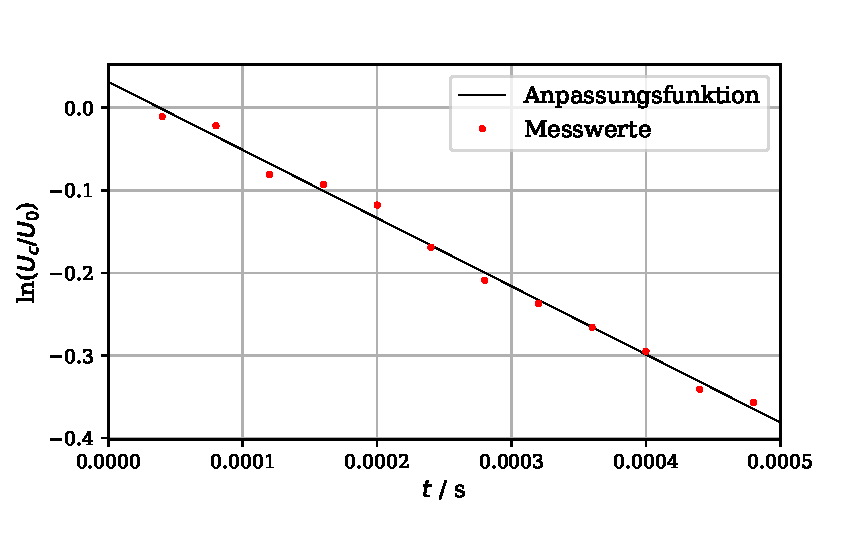
\includegraphics{plot1.pdf}
  \caption{Logarithmus der Kondensatorspannung in Abhängigkeit der Zeit.}
  \label{fig:plot}
\end{figure}
\noindent Um die Ausgleichsgerade zu bestimmen, wird Gleichung (4) entsprechend umgeformt:
\begin{align*}
    \frac{U_c}{U_0} = e^{-\frac{t}{RC}}
\end{align*}
\begin{equation*}
    \leftrightarrow ln{(\frac{U_c}{U_0})} = -\frac{1}{RC}t .
\end{equation*}
Somit hat die Gerade folgende Gestalt:
\begin{equation}
    ln{(\frac{U_c}{U_0})} = \underbrace{-\frac{1}{RC}}_{Steigung \: a}t + b .
\end{equation}
Daraus ergeben sich $a = (-824.913 \pm 20.909)\si{\second}$ und $b = (3.123 \pm 0.616) \cdot 10^{-2} $ .
Daraus folgt für $RC$:
\begin{equation*}
    RC = -\frac{1}{a} = (1.21 \pm 0.04)\cdot 10^{-3} \si{\second} , 
\end{equation*}
wobei der Fehler berechnet wird mit
\begin{equation*}
   \Delta RC = \sqrt{(\frac{dRC}{da})^2\Delta a^2} = \sqrt{(\frac{1}{a^2})^2 \Delta a^2} ,
\end{equation*}
mit $\Delta a$ als der oben aufgelistete Fehler des Parameters $a$.

\begin{table}[H]
  \centering
  \caption{Gemessene Spannung und Logarithmus der Spannung zum Zeitpunkt $t$ beim Entladevorgang des Kondensators. }
  \label{tab:Parameter}
  \begin{tabular}{c c c}
    \toprule
    $t\cdot 10^{-3}/$s & $U_c/$V & $ln(U_c/U_0)$  \\
    \bottomrule
     0.04 & 17.8  & -0.011 \\
     0.08 & 17.6  & -0.022\\
     0.12& 16.6  & -0.081\\
     0.16& 16.4  & -0.093\\
     0.20 & 16.0  &-0.118\\
     0.24 & 15.2  &-0.169\\
     0.28 & 14.6  &-0.209\\
     0.32& 14.2 & -0.237\\
     0.36& 13.8  & -0.266\\
     0.40& 13.4  & -0.295\\
     0.44& 12.8  & -0.341\\
     0.48& 12.6  & -0.357\\
     
    \bottomrule
  \end{tabular}
\end{table}

\subsection{Bestimmung der Zeitkonstanten durch die Frequenz der Kondensatorspannung}
Die für diese Methode gemessenen Daten finden sich in Tabelle (2). 
In einem halblogarithmischen Diagramm wird die Amplitude gegen die Frequenz aufgetragen.

\begin{figure}[H]
  \centering
  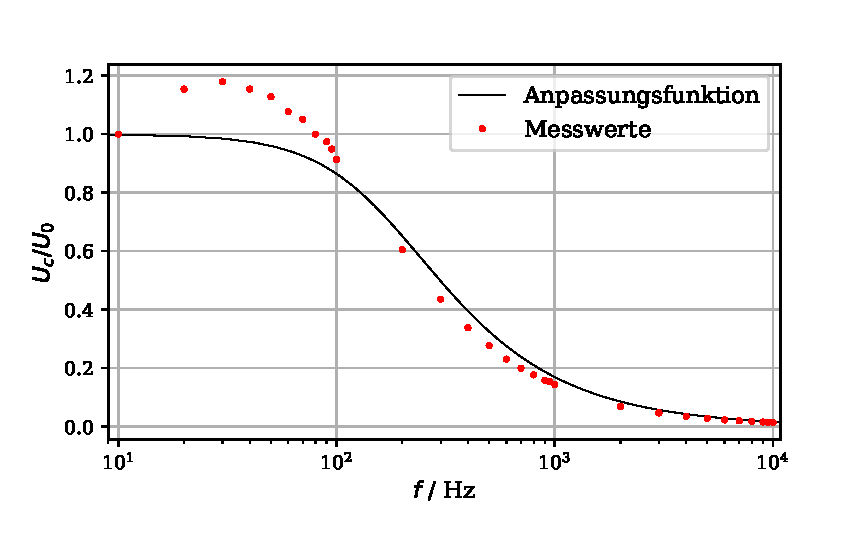
\includegraphics{plot2.pdf}
  \caption{Kondensatorspannung in Abhängigkeit der Frequenz.}
  \label{fig:plot}
\end{figure}

\noindent Die Ausgleichsgleichung hat folgende Gestalt
\begin{equation*}
    \frac{A(\omega)}{U_0} = \frac{1}{ \sqrt{1+\omega^2R^2C^2}} ,
\end{equation*}
was sich aus Gleichung (9) ergibt. $U_0$ beträgt hierbei 7.8 Volt. Da die Amplitude aus der Gleichung von der Kreisfrequenz abhängt, 
muss für die Ausgleichsrechnung noch ein Faktor $2\pi$ beachtet werden, auf Grund des Zusammenhangs
\begin{equation}
    \omega = 2\pi f .
\end{equation}
Somit wird der Graph durch
\begin{equation}
    y = \frac{1}{ \sqrt{1+d^2(2\pi f)^2}} 
\end{equation}
beschrieben.
Der Parameter lautet:
\begin{align*}
   d = RC = (0.9256\pm  0.0785)\cdot 10^{-3} \si{\second} .
\end{align*}


\begin{table}[H]
\small
  \centering
  \caption{Gemessene Amplituden und Phasenverschiebung bei unterschiedlicher Frequenz.}
  \label{tab:Parameter}
  \begin{tabular}{c c c c c c c c c c}
    \toprule
    $f/$Hz & $U/$V & $a/$s & $T/s^{-1}$ & $\phi/$rad & $f/$Hz & $U/$V & $a/$s & $T/s^{-1}$ & $\phi/$rad \\
    \bottomrule
     10  & 7.8  & 0.00156 & 0.1 & 0.098 & 600 & 1.8 & 0.00036 & 0.0017 & 1.35 \\
     20  & 9 & 0.00144 & 0.05 & 0.181 & 700 & 1.56 & 0.00031 & 0.0014 & 1.138\\
     30  & 9.2& 0.0014 & 0.033 & 0.264 & 800 & 1.38 & 0.00028 & 0.0013 & 1.39\\
     40  & 9 & 0.00134 & 0.025 & 0.337 & 900 & 1.24 & 0.00025 & 0.0011 & 1.4\\
     50  & 8.8 & 0.00132 & 0.02 & 0.415 & 950 & 1.2 & 0.00024 & 0.0011 & 1.43\\
     60  & 8.4 & 0.0013 & 0.017 & 0.49 & 1000  & 1.12 & 0.00022 & 0.001 & 1.41\\
     70  & 8.2 & 0.00126 & 0.014 & 0.554 & 2000  & 0.54 & 0.00012 & 0.0005 & 1.47\\
     80  & 7.8 & 0.00122 & 0.013 & 0.613 & 3000  & 0.36 & 0.00008 & 0.0003 & 1.52\\
     90  & 7.6 & 0.00119 & 0.011 & 0.67 & 4000  & 0.28 & 0.00006 & 0.0003 & 1.52\\
     95  & 7.4 & 0.00117 & 0.011 & 0.698 & 5000  & 0.22 & 0.000048 & 0.002 & 1.52 \\
     100 & 7.12 & 0.00115 & 0.01 & 0.723 & 6000 & 0.18 & 0.00004 & 0.0002 & 1.54\\
     200 & 4.72 & 0.00083 & 0.005 & 1.046 & 7000  & 0.16 & 0.000035 & 0.0001 & 1.52\\
     300 & 3.4 & 0.00064 & 0.003 & 1.199 & 8000  & 0.14 & 0.00003 & 0.0001 & 1.5\\
     400 & 2.64 & 0.0005 & 0.003 & 1.277 & 9000  & 0.12 & 0.000027 & 0.0001 & 1.55\\
     500 & 2.16 & 0.00042 & 0.002 & 1.332 & 9500  & 0.12 & 0.000026 & 0.0001 & 1.53\\
     10000 & 0.112 & 0.00002 & 0.0001 & 1.533\\
    \bottomrule
  \end{tabular}
\end{table}
\noindent Die Werte für $\phi$ wurden dabei mit Gleichung (6) berechnet, wobei $b$ als Kehrwert der Frequenz berechnet wird.


\subsection{Bestimmung der Zeitkonstanten durch die Phasenverschiebung zwischen Generator- und Kondensatorspannung}
In diesem Auswertungsteil wird wie in 3.2 verfahren, nur dass die Phasenverschiebung gegen die Frequenz aufgetragen wird.
Die dafür benötigten Werte sind in Tabelle (2) aufgelistet.

\noindent Aus Gleichung (16) ergibt sich der Ansatz für diesen Graphen:
\begin{equation}
    y = arctan(2 \pi f  d) .
\end{equation}
\begin{figure}[H]
  \centering
  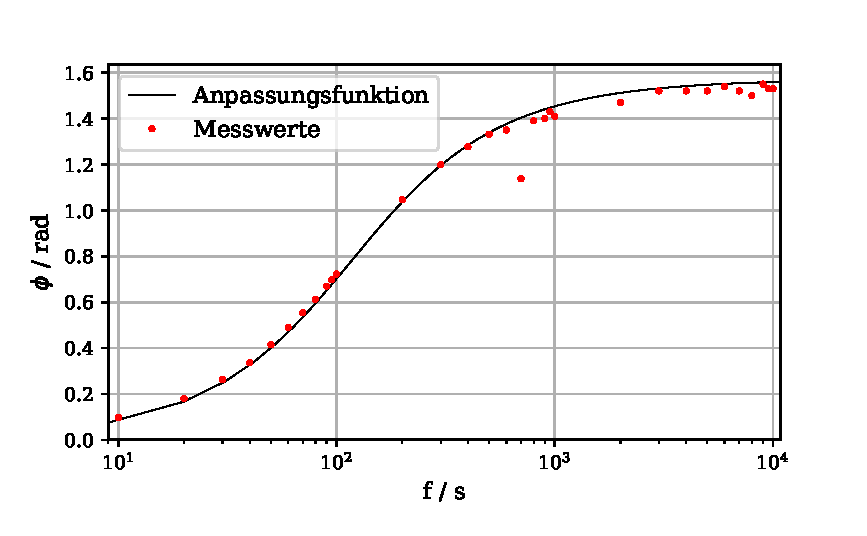
\includegraphics{plot3.pdf}
  \caption{Phasenverschiebung in Abhängigkeit der Frequenz.}
  \label{fig:plot}
\end{figure}
\noindent Die Zeitkonstante beträgt:
\begin{align*}
   d = RC = (1.346 \pm 0.498) \cdot 10^{-3} \si{\second} .
\end{align*}



\noindent Die Relativamplitude $U_c/U_0$ wird gegen die Phasenverschiebung in einem Polarplot aufgetragen.
Mit der Gleichung
\begin{equation*}
    \frac{A(f)}{U_0} = -\frac{sin \phi}{2\pi f RC} 
\end{equation*}
kann eine Kosinus-Abhängigkeit hergeleitet werden, da
\begin{equation*}
    \frac{sin\phi}{cos\phi} = -\omega RC 
\end{equation*}
gilt. Dies führt auf
\begin{equation}
    \frac{A(f)}{U_0} = cos\phi .
\end{equation}

\noindent Die Kurve dazu wird mit Python berechnet.
\begin{figure}[H]
  \centering
  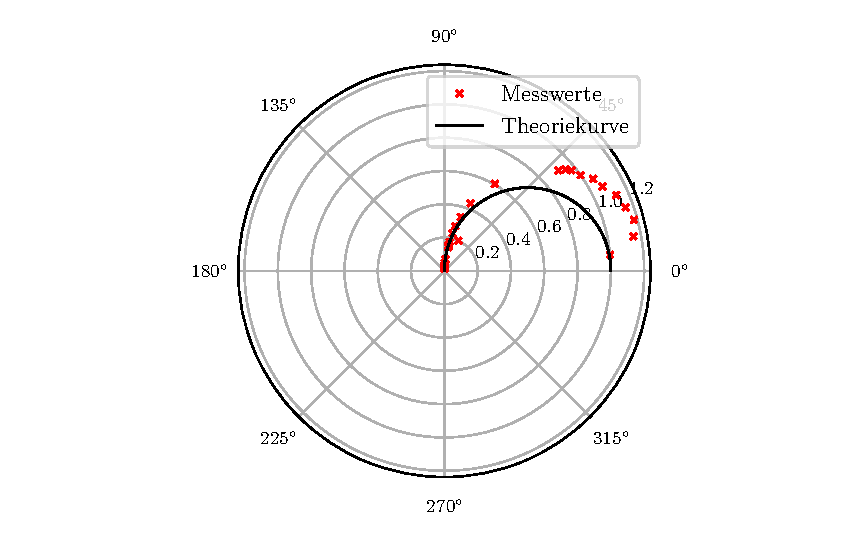
\includegraphics{plot4.pdf}
  \caption{Abhängigkeit der Amplitude und Phase in einem Polarplot.}
  \label{fig:plot}
\end{figure}

\subsection{RC-Kreis als Integrator}
\noindent Zuletzt wird geprüft, ob der RC-Kreis als Integrator arbeiten kann.

\begin{figure}[H]
  \centering
  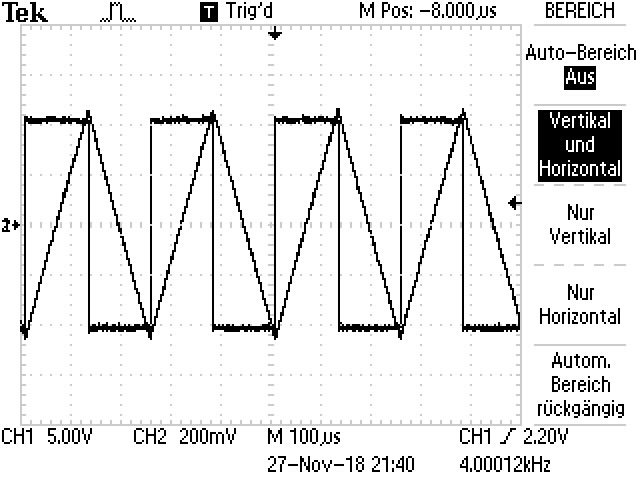
\includegraphics{Rechteck.JPG}
  \caption{Darstellung der Rechtecktspannung und ihrer Integrierten in einem Oskilloskop-Druck.}
  \label{fig:plot}
\end{figure}
\noindent Wie zu erkennen ist, ist die Integrierte einer Rechteckspannung eine Dreieckspannung.
Folgende konstane Funktion
\begin{equation*}
  f(t) =
  \begin{cases}
    U & \text 0 < t < a \\
    -U & \text a < t < 2a \\
  \end{cases}
\end{equation*}
liefert diese Stammfunktion:
\begin{equation*}
  F(t) =
  \begin{cases}
    Ut & \text 0 < t < a \\
    -Ut & \text a < t < 2a .\\
  \end{cases}
\end{equation*}

\begin{figure}[H]
  \centering
  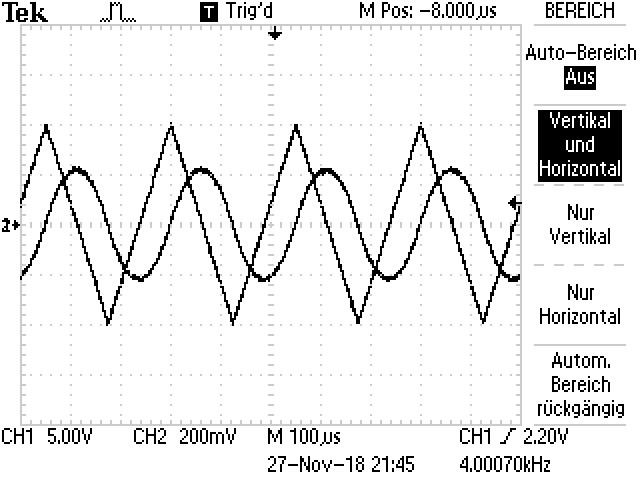
\includegraphics{Dreieck.JPG}
  \caption{Darstellung der Dreiecksspannng und ihrer Integrierten in einem Oszilloskop-Druck.}
  \label{fig:plot}
\end{figure}

\noindent Bei einer Dreieckspannung ist eine quadratische Funktion die Integrierte.
Die Funktion
\begin{equation*}
  f(x) =
  \begin{cases}
    Ux & \text 0 < x < a \\
    -Ux & \text a < x < 2a \\
  \end{cases}
\end{equation*}
ergibt integriert:
\begin{equation*}
  F(x) =
  \begin{cases}
    \frac{1}{2} \cdot Ux^2 & \text 0 < x < a \\
    -\frac{1}{2} \cdot Ux^2 & \text a < x < 2a .\\
  \end{cases}
\end{equation*}
\begin{figure}[H]
  \centering
  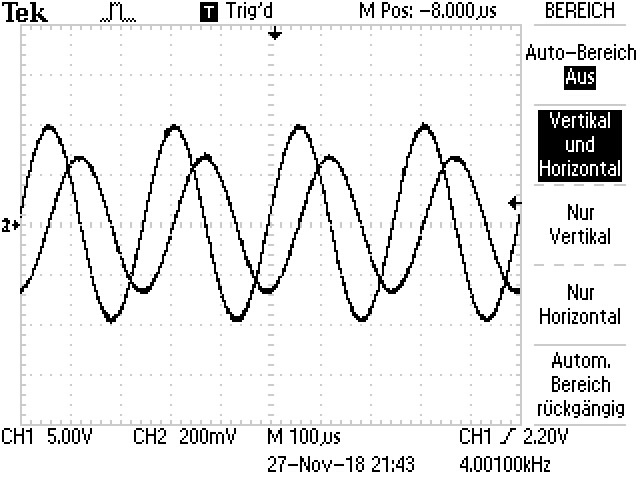
\includegraphics{Sinus.JPG}
  \caption{Darstellung der Sinusspannung und ihrer Integrierten in einem Oszilloskop-Druck.}
  \label{fig:plot}
\end{figure}
\noindent Eine Kosinusspannung ist die Integrierte der Sinusspannung.
Die Stammfunktion einer Sinusfunktion lautet
\begin{equation*}
  F(x) = -U \cdot cos(x) .
\end{equation*}



